
\section{Maximum Likelihood}
\begin{enumerate}
\item Generate equiprobable $X \in \cbrak{1,-1}$.\\
\solution $X$ can be generated in python using the below code section,
\begin{lstlisting}
	chapter3/codes/eqi_prob.py
\end{lstlisting}
\item Generate 
\begin{equation}
Y = AX+N,
\end{equation}
where $A = 5$ dB,  and $N \sim \gauss{0}{1}$.\\
\solution $Y$ can be generated in python using the below code section,
\begin{lstlisting}
	chapter3/codes/Y_gau.py
\end{lstlisting}
\item Plot $Y$ using a scatter plot.\\
\solution 
\begin{lstlisting}
		chapter3/codes/scatter.py
\end{lstlisting}
\begin{figure}[H]
\centering
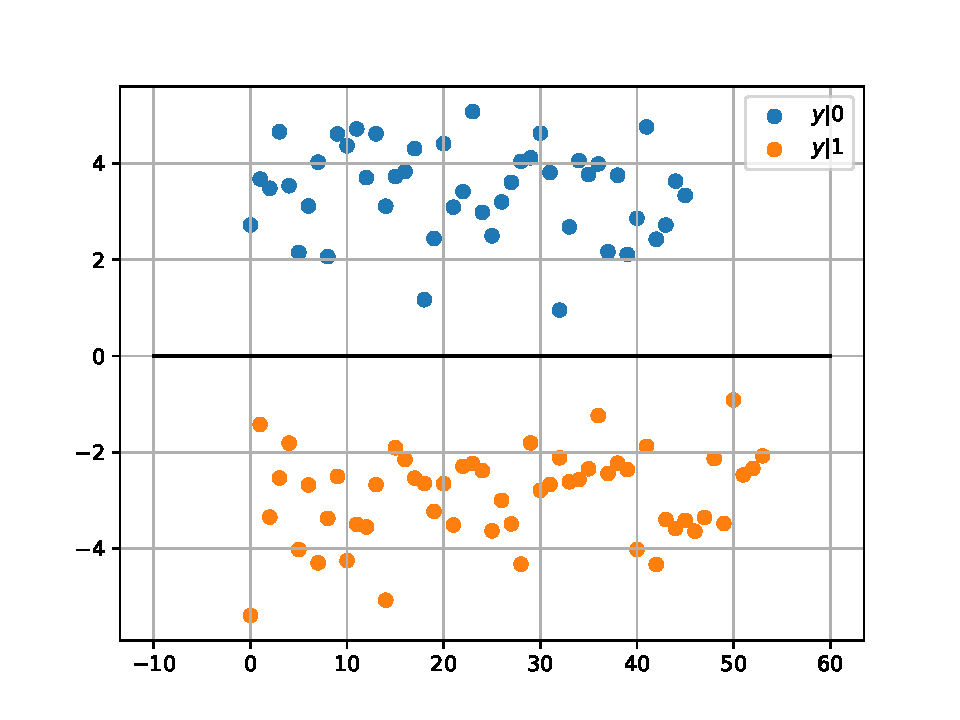
\includegraphics[width=\columnwidth]{chapter3/figs/bpsk_scatter.pdf}
\caption{Scatter plot of $Y$}
\label{fig:bpsk_scatter}
\end{figure}
\item Guess how to estimate $X$ from $Y$.\\
\solution
\begin{equation}
y \dec{1}{-1} 0
\label{eq:bpsk_decision}
\end{equation}
\item
\label{ml-ch4_sim}
Find 
\begin{equation}
	P_{e|0} = \pr{\hat{X} = -1|X=1}
\end{equation}
and 
\begin{equation}
	P_{e|1} = \pr{\hat{X} = 1|X=-1}
\end{equation}\\
\solution
\begin{flalign*}
	\pr{\hat{X} = -1|X=1} &= \pr{Y < 0|X=1}&\\
	&= \pr{AX + N < 0|X=1}&\\ 
	&= \pr{A + N < 0}&\\
	&= \pr{N < -A}
\end{flalign*}
Similarly,
\begin{flalign*}
	\pr{\hat{X} = 1|X=-1} &= \pr{Y > 0|X=-1}&\\
	&= \pr{N > A}
\end{flalign*}
Since $N \sim \gauss{0}{1}$,
\begin{flalign}
	\label{eq:std_norm_symmetric}
	\pr{N < -A} &= \pr{N > A}&\\
	\label{eq:bpks_prob_err_cond}
	\implies P_{e|0} &= P_{e|1} = \pr{N > A}
\end{flalign}
%
\item Find $P_e$ assuming that $X$ has equiprobable symbols.\\
\solution
\begin{flalign}
	P_e &= \pr{X=1}P_{e|1} + \pr{X=-1}P_{e|0}&\\
	\intertext{Since $X$ is equiprobable}\\
	\label{eq:bpsk_prob_error_equi}
	P_e &= \frac{1}{2}P_{e|1} + \frac{1}{2}P_{e|0}
\end{flalign}
Substituting from \eqref{eq:bpks_prob_err_cond}
\begin{equation}
	P_e = \pr{N > A}
\end{equation}
Given a random varible $X \sim \gauss{0}{1}$ the Q-function is defined as
\begin{align}
	Q(x) &= \pr{X > x}\\
	\label{eq:q_func_integral}
	Q(x) &= \frac{1}{\sqrt{2\pi}} \int_x^\infty \exp\left(-\frac{u^2}{2}\right) \, du.\\
\end{align}
Using the Q-function, $P_e$ is rewritten as
\begin{equation}
	P_e = Q(A)
\end{equation} 
%
\item
Verify by plotting  the theoretical $P_e$ with respect to $A$ from 0 to 10 dB.\\
\solution 
\begin{lstlisting}
		chapter3/codes/bpsk_pe.py
\end{lstlisting}
\begin{figure}[H]
\centering
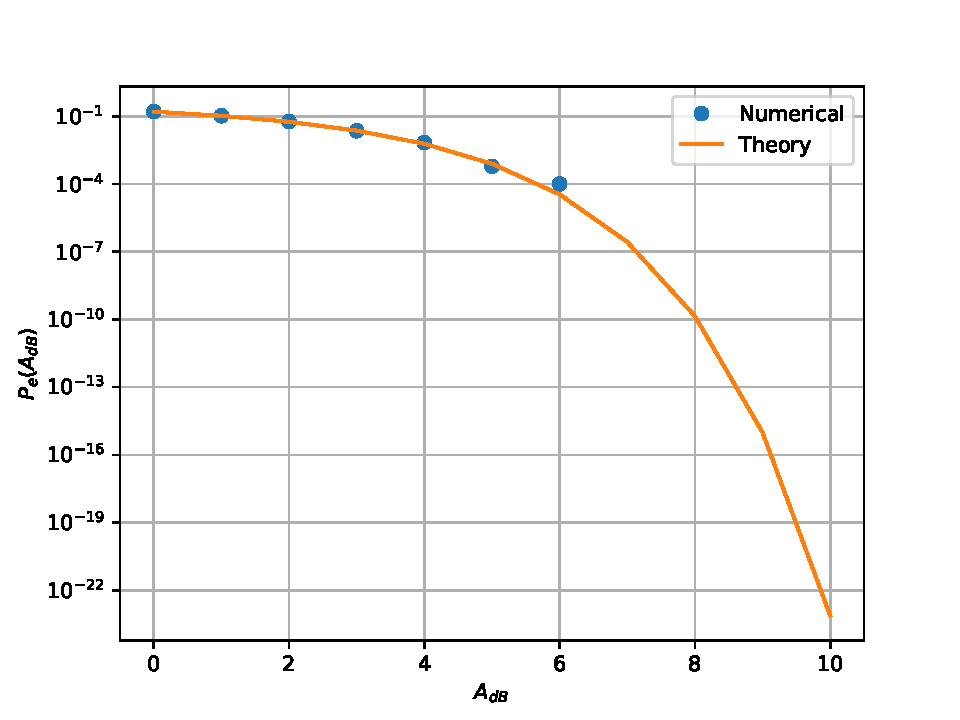
\includegraphics[width=\columnwidth]{chapter3/figs/bpsk_pe_snr.pdf}
\caption{$P_e$ versus $A$ plot}
\label{fig:bpsk_pe_snr}
\end{figure}
%
\item Now, consider a threshold $\delta$  while estimating $X$ from $Y$. Find the value of $\delta$ that maximizes the theoretical $P_e$.\\
\label{prob:bpsk_delta_equi}
\solution Given the decision rule, 
\begin{equation}
y \dec{1}{-1} \delta
\label{eq:bpsk_decision_delta}
\end{equation}
\begin{flalign*}
	P_{e|0} &= \pr{\hat{X} = -1|X=1}&\\
	&= \pr{Y < \delta|X=1}&\\
	&= \pr{AX + N < \delta|X=1}&\\ 
	&= \pr{A + N < \delta}&\\
	&= \pr{N < -A + \delta}&\\
	&= \pr{N > A - \delta}&\\
	&= Q(A-\delta)
\end{flalign*}
\begin{flalign*}
	P_{e|1} &= \pr{\hat{X} = 1|X=-1}&\\
	&= \pr{Y > \delta|X=-1}&\\
	&= \pr{N > A + \delta}&\\
	&= Q(A+\delta)
\end{flalign*}
Using \eqref{eq:bpsk_prob_error_equi}, $P_e$ is given by
\begin{flalign}
	P_e &= \frac{1}{2}Q(A+\delta) + \frac{1}{2}Q(A-\delta)
\end{flalign}
Using the integral for Q-function from \eqref{eq:q_func_integral},
\begin{align}
	\label{eq:prob_error_delta_equi}
	P_e &= k(\int_{A+\delta}^\infty \exp\left(-\frac{u^2}{2}\right) \, du + \int_{A-\delta}^\infty \exp\left(-\frac{u^2}{2}\right) \, du)\\
	\intertext{where k is a constant}	\nonumber
\end{align}
Differentiating \eqref{eq:prob_error_delta_equi} wrt $\delta$ (using Leibniz's rule) and equating to $0$, we get
\begin{flalign*}
	\exp\left(-\frac{(A+\delta)^2}{2}\right)-\exp\left(-\frac{(A-\delta)^2}{2}\right) &= 0&\\
	\frac{\exp\left(-\frac{(A+\delta)^2}{2}\right)}{\exp\left(-\frac{(A\delta)^2}{2}\right)} &= 1&\\
	\exp\left(-\frac{(A+\delta)^2-(A-\delta)^2}{2}\right) &= 1&\\
	\exp\left(-2A\delta\right) &= 1&\\
	\intertext{Taking $\ln$ on both sides}\\
	-2A\delta &= 0&\\
	\implies \delta &= 0
\end{flalign*}
$P_e$ is maximum for $\delta = 0$
\item Repeat the above exercise when 
\label{prob:bpsk_decision_uneqi}
	\begin{align}
		p_{X}(0) = p
	\end{align}\\
\solution Since $X$ is not equiprobable, $P_e$ is given by,
\begin{flalign}
	P_e &= (1-p)P_{e|1} + pP_{e|0}&\\
	&= (1-p)Q(A+\delta) + pQ(A-\delta)
\end{flalign}
Using the integral for Q-function from \eqref{eq:q_func_integral},
\begin{multline}
	\label{eq:prob_error_delta_nonequi}
	P_e = k((1-p)\int_{A+\delta}^\infty \exp\left(-\frac{u^2}{2}\right) \, du + \\
	p\int_{A-\delta}^\infty \exp\left(-\frac{u^2}{2}\right) \, du)
\end{multline}
where $k$ is a constant.\\
Following the same steps as in problem \ref{prob:bpsk_delta_equi}, $\delta$ for maximum $P_e$ evaluates to,
\begin{equation}
	\delta = \frac{1}{2A}\ln\left(\frac{1}{p}-1\right)
\end{equation}
\item Repeat the above exercise using the MAP criterion.\\
\solution 
The MAP rule can be stated as\\
\begin{flalign}
\label{eq:map_rule}
\text{Set } \hat{x} &= x_i \text{ if}&\\ \nonumber
p_X(x_k)p_Y(y|x_k) &\text{ is maximum for } k = i
\end{flalign}
For the case of BPSK, the point of equality between $p_X(x=1)p_Y(y|x=1)$ and $p_X(x=-1)p_Y(y|x=-1)$ is the optimum threshold. If this threshold is $\delta$, then
\begin{flalign*}
	pp_Y(y|x=1) > (1-p)p_Y(y|x=-1) &\text{ when } y > \delta&\\
	pp_Y(y|x=1) < (1-p)p_Y(y|x=-1) &\text{ when } y < \delta 	
\end{flalign*}
The above inequalities can be visualized in \figref{fig:bpsk_map_density} for $p = 0.3$ and $A = 3$.
\begin{figure}[H]
\centering
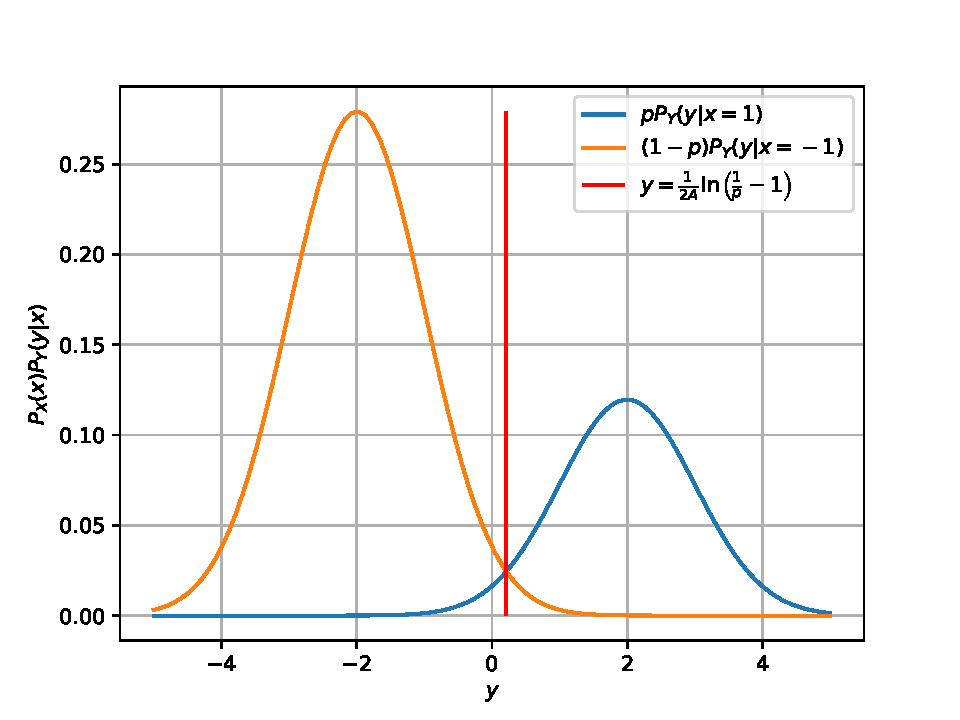
\includegraphics[width=\columnwidth]{chapter3/figs/bpsk_map_density.pdf}
\caption{$p_X(X=x_i)p_Y(y|x=x_i)$ versus $y$ plot for $X \in \{-1,1\}$}
\label{fig:bpsk_map_density}
\end{figure}
Given $Y=AX+N$ where $N \sim \gauss{0}{1}$, the optimum threshold is found as solution to the below equation
\begin{equation}
	p\exp\left(-\frac{(y_{eq}-A)^2}{2}\right) = (1-p)\exp\left(-\frac{(y_{eq}+A)^2}{2}\right)
\end{equation}
Solving for $y_{eq}$, we get
\begin{equation}S
	y_{eq} = \delta = \frac{1}{2A}\ln\left(\frac{1}{p}-1\right)
\end{equation}
which is same as $\delta$ obtained in problem \ref{prob:bpsk_decision_uneqi}

\begin{lstlisting}
		chapter3/codes/map.py	
\end{lstlisting}
\end{enumerate}-
